\documentclass[a4paper]{report}
\usepackage{a4wide}
\usepackage[utf8]{inputenc}
\usepackage{parskip}
\usepackage{hyperref}
\usepackage{epsfig}
\usepackage{background}
\usepackage{mathptmx}

% To avoid tikz error, see https://tex.stackexchange.com/questions/165929/semiverbatim-with-tikz-in-beamer
\makeatletter
\global\let\tikz@ensure@dollar@catcode=\relax
\makeatother

\backgroundsetup{
scale=1,
angle=0,
opacity=1,
contents={
\includegraphics[width=\paperwidth,height=\paperheight]{images/spi-front.jpg}}
}

\hypersetup{
  colorlinks   = true,
  urlcolor     = blue,
  linkcolor    = blue,
  pdfinfo = {
    Title = {SPI Annual Report 2017},
    Author = {Software in the Public Interest, Inc.},
    Keywords = {SPI, free software, open source, FOSS, annual report, charity, non-profit, 501c3},
  }
}

\begin{document}

\title{Software in the Public Interest, Inc.\\
2017 Annual Report}
\date{July 23, 2018}

\maketitle

\newpage

\backgroundsetup{
scale=1,
angle=0,
opacity=1,
contents={
\includegraphics[width=\paperwidth,height=\paperheight]{images/spi-content.jpg}}
}

\hspace{1em}

To the membership, board and friends of Software in the Public Interest, Inc:

As mandated by Article 8 of the SPI Bylaws, I respectfully submit this annual
report on the activities of Software in the Public Interest, Inc. and extend my
thanks to all of those who contributed to the mission of SPI in the past year.

  \emph{-- Martin Michlmayr, SPI President}

\newpage

\tableofcontents

\newpage

\chapter{President's Welcome}
\label{sec:president}

SPI has served the free and open source software community for over 20
years since our establishment in 1997.  SPI was founded by contributors
to the Debian project with the vision to start an organization that can
serve the wider free software community.  With 45 associated projects,
we have fulfilled this vision.  We've also made some progress in getting
a more diverse board and attracting directors from SPI associated
projects other than Debian.

SPI now holds over 850,000 dollars in trust for SPI associated projects.
This is a great responsibility which requires diligence from our
organization.  It's important for us to acknowledge the trust placed in
us by SPI associated projects and to improve the governance and
operations of SPI even further.  We've made good progress improving our
accounting processes and we continue to work on this.

SPI and its associated projects have accomplished much in the first 20
years, and we intend to operate for a long time to come.  This is thanks
to the board, our members, volunteers of SPI and its associated projects
and to many generous sponsors.  Thank you to all of you!

  \emph{-- Martin Michlmayr, SPI President}

\chapter{Committee Reports}
\section{Membership Committee}

\subsection{Statistics}

On January 1, 2017 we had 246 contributing and 900 non-contributing
members.  On December 31, 2017 there were 255 contributing members and
960 non-contributing members.

\chapter{Board Report}
\section{Board Members}

Board members as of January 1, 2017:

\begin{itemize}
\item Martin Michlmayr (President)
\item Joerg Jaspert (Vice President)
\item Valerie Young (Secretary)
\item Michael Schultheiss (Treasurer)
\item Luca Filipozzi
\item Jimmy Kaplowitz
\item Dimitri John Ledkov
\item Andrew Tridgell
\item Martin Zobel-Helas
\end{itemize}

Board members as of December 31, 2017:

\begin{itemize}
\item Martin Michlmayr (President)
\item Luca Filipozzi (Vice President)
\item Valerie Young (Secretary)
\item Michael Schultheiss (Treasurer)
\item Joerg Jaspert
\item Jimmy Kaplowitz
\item Tim Potter
\item Andrew Tridgell
\item Martin Zobel-Helas
\end{itemize}

Advisors to the board as of December 31, 2017:

\begin{itemize}
\item Software Freedom Law Center (SFLC), legal counsel
\item Chris Lamb, Debian Project representative
\item Robert Treat, PostgreSQL Project representative
\end{itemize}

\section{Board Changes}

Changes that occurred during the year:

\begin{itemize}

\item Dimitri John Ledkov resigned from the board in July 2017 due to lack
of time.  We'd like to thank Dimitri for his contributions!

\item Andrew Tridgell generously offered to resign early to reset the
election of board members to three per year. SPI typically elects three
(out of nine) board members each year but this got out of sync over the
years.

\item The term for Martin Michlmayr expired in July 2017.

\item Tridgell and Michlmayr sought, and obtained, re-election.  Tim
Potter joined the board as part of the same election.

\item On August 14, 2017 the board voted to appoint the following
officers:

\begin{itemize}
\item President: Martin Michlmayr
\item Vice President: Luca Filipozzi
\item Secretary: Valerie Young
\item Treasurer: Michael Schultheiss
\end{itemize}

\end{itemize}

\section{Elections}

A board membership election was conducted in July 2017.  There were 3 board
seats up for election.  Nominations were received from Martin Michlmayr,
Tim Potter, and Andrew Tridgell.  Since there were 3 nominations for 3
board seats, no vote was required and Martin Michlmayr, Tim Potter, and
Andrew Tridgell were elected for a 3 year term.

\section{Face-to-face Meetings}

The SPI board held a face-to-face meeting on February 24-25, 2017.
The meeting was held at the Software Freedom Law Center (SFLC) in New
York.

A second face-to-face meeting was held on October 13-14, 2017.

We discussed many topics, including new by-laws, our financial system,
and mission and roadmap.

In the future, one face-to-face meeting will be held in the fall (a few
months after the board election in July).  An annual face-to-face
meeting helps with the onboarding of new directors and more generally
with board engagement and is used to set the agenda for the remainder
of the year and the following year.

\begin{figure*}[h]
\centering

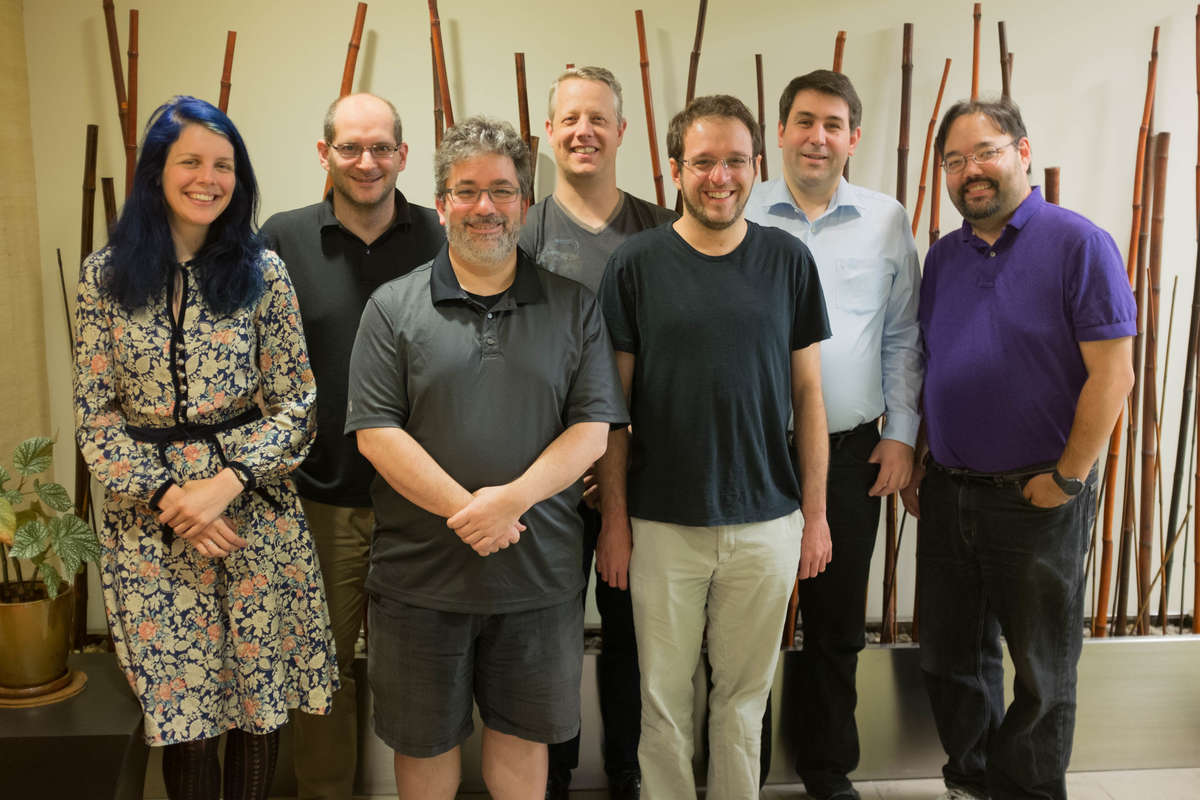
\includegraphics[scale=1.00]{images/2017-october-f2f}

\caption{Face-to-face meeting in New York (October 2017): Valerie Young,
Martin Michlmayr, Luca Filipozzi, Tim Potter, Jimmy Kaplowitz, Martin
Zobel-Helas and Michael Schultheiss (left to right)}

\end{figure*}

\section{Improvements to Operations}

SPI signed up for a virtual mailbox with an address in New York (to
match our jurisdiction).  This service offers physical-to-virtual mail
forwarding and cheque-deposit (to aid with timely response to snail
mail).  This makes SPI less reliant on a specific person to check a
physical mailbox.

SPI signed up for a virtual phone number so that we have one official
phone number.  This allows us, for example, to respond to identity
checks for things like Extended Validation SSL Certificates.

SPI engaged a contract employee to aid with incoming treasurer requests.
The contractor helped with DebConf17 reimbursements (ensuring that all
requests, including receipts, are complete).  We intend to use this
contractor for more ticket triage in the future and possibly extend the
help more widely to other accounts tasks involving account receivable
(AR) and accounts payable (AP).

\chapter{Treasurer's Report}

This report uses a cash-based method of accounting, recording donations when
deposited (not when the check was written or received by us) and recording
expenses when sent or scheduled for payment (not when incurred).

\section{Income Statement}

This covers the Period January 1, 2017 -- December 31, 2017

\begin{verbatim}
 Income
   Ordinary Income
        0 A.D.                           2,963.58
        Ankur                                9.53
        Aptosid                             97.85
        Arch Linux                      21,423.79
        ArduPilot                       31,182.32
        Chakra                             658.82
        DebConf16                        4,750.00
        DebConf17                      135,481.03
        Debian                          41,728.94
        FFmpeg                           9,251.55
        FFmpeg (OPW)                       361.95
        Fluxbox                              2.85
        freedesktop.org                    541.50
        FreedomBox Foundation               28.50
        Gallery                              0.00
        GNU TeXmacs                         26.80
        GNUstep                              0.00
        haskell.org                        617.50
        Jenkins                          6,600.71
        LibreOffice                     24,962.69
        MinGW                               58.52
        NTPsec                         190,027.55
        Open Bioinformatics              9,694.27
        Open MPI                           546.26
        Open Voting Foundation              28.50
        OpenEmbedded                       114.02
        OpenVAS                              9.50
        OpenWrt                            309.26
        OpenZFS                         33,740.39
        OSUNIX                               0.00
        Performance Co-Pilot             5,414.95
        PostgreSQL                      34,051.80
        Privoxy                          2,509.30
        Swathanthra Malayalam Computing      0.00
        SPI General                     68,845.81
        The HeliOS Project                   0.00
        Tux4Kids                            20.90
        X.Org                            7,048.05
        YafaRay                          1,900.00

        Total Ordinary Income          635,008.99
                                       ----------
   Interest Income
        Ameriprise Brokerage                37.56
        Key Business Platinum MM Savings    24.40
        Chase BusSelect High Yield Savings 198.02
        Fifth Third Business MM 128         42.62

        Total Interest Income              302.60
                                           ------

   Gross Income                        635,311.59
                                       ----------

 Expenses
  Ordinary Expenses

        0 A.D.
          164.88    Banking fees
        1,043.65    IT
        --------
        1,208.53

        Ankur
            0.82    Banking fees

        Aptosid
            5.02    Banking fees

        Arch Linux
          813.11    Banking fees
           35.00    Chargeback
        3,549.05    IT
        --------
        4,397.16

        ArduPilot
          878.46    Banking fees
       14,448.23    Development
        3,315.44    IT
          615.02    Meetups
       ---------
       19,257.15

        Chakra
           27.13    Banking fees
          450.00    Office
          ------
          477.13

        DebConf 15
        1,065.29    Meetups

        DebConf 16
          145.30    Banking fees
        4,037.09    Meetups
        --------
        4,182.39

        DebConf 17
          350.35    Banking fees
            8.22    IT
      182,157.00    Meetups
          304.66    Office
      ----------
      182,820.23

        Debian
        1,700.21    Banking fees
       19,500.00    Development
       (1,723.93)   IT (Refund)
       25,349.02    Meetups
       ---------
       44,825.30

        Drizzle
          185.39    IT

        FFmpeg
          155.18    Banking fees
        7,505.01    Development
        3,844.34    Meetups
          513.70    Office
       ---------
       12,018.23

        FFmpeg (OPW)
           18.04    Banking fees

        Fluxbox
            0.71    Banking fees

        freedesktop.org
           22.98    Banking fees
          300.00    Development
        2,452.56    Meetups
        ---------
        2,775.54

        FreedomBox Foundation
            1.90    Banking fees
       25,053.00    Transfer to FreedomBox Foundation
       ---------
       25,054.90

        Gallery
        8,357.68    IT

        GNU TeXmacs
            2.36    Banking fees

        haskell.org
           28.10    Banking fees
           85.47    IT
          ------
          113.57

        Jenkins
          281.85    Banking fees
          388.60    Development
        3,693.65    Meetups
         -------
        4,364.10

        LibreOffice
          135.75    Banking fees
       46,590.52    Meetups
       ---------
       46,726.27

        MinGW
            4.83    Banking fees

        NTPsec
            1.53    Banking fees
      184,000.00    Development
      ----------
      184,001.53

        Open Bioinformatics
           41.23    Banking fees
          209.41    IT
          735.85    Meetups
          ------
          986.49

        OpenEmbedded
            6.26    Banking fees

        Open MPI
            0.01    Banking fees

        Open Voting Foundation
            1.49    Banking fees

        OpenVAS
            0.67    Banking fees

        OpenWrt
           16.20    Banking fees

        OpenZFS
          642.81    Banking fees
       32,772.44    Meetups
          442.89    Office
       ---------
       33,858.14

        Performance Co-Pilot
            0.30    Banking fees
        1,525.00    Meetups
        --------
        1,525.30

        PostgreSQL
          236.94    Banking fees
        5,000.00    Development
        1,841.78    Meetups
          129.00    Office
        --------
        7,207.72

        privoxy
           71.62    Banking fees
          916.06    IT
          ------
          987.68

        Swathanthra Malayalam Computing
            0.30    Banking fees

        SPI
        1,244.25    Banking fees
           88.01    Chargeback
       20,146.50    Meetups
        2,408.99    Office
       ---------
       23,887.75

        Tux4Kids
            1.38    Banking fees

        X.Org
           43.48    Banking fees
        1,668.86    Meetups
          113.75    Office
        --------
        1,826.09

        YafaRay
           80.35    Office
          693.09    IT
          ------
          773.44

        Total Expenses          612,941.09
                                ----------

        Net Income               22,370.50
\end{verbatim}

\section{Balance Sheet}

\begin{verbatim}
Balance Sheet as of December 31, 2017

   ASSETS
     Current Assets
        Ameriprise Cash Mgmt Acct                         13,443.71
        Chase Business Select High Yield Savings         170,225.61
        Chase Performance Business Checking              138,443.58
        Fifth Third Business Elite Checking (Debian)      86,334.51
        Fifth Third Business Elite Checking (SPI)         30,151.69
        Fifth Third Business Elite Checking Wiretransfer 124,561.81
        Fifth Third Business Money Market 128             30,004.92
        KeyBank Basic Business Checking                    8,922.08
        Key Business Platinum Money Market Savings       112,940.87
        Key Business Reward Checking                     343,331.32
        Key Express Checking (closed)                          0.00
        Debian Debit Card (closed)                             0.00
        PayPal (Debian)                                    1,637.75
        PayPal (SPI)                                      17,244.21
        Bank transfers in progress                         6,000.00

     Total Current Assets                              1,083,242.06

   TOTAL ASSETS                                        1,083,242.06

   LIABILITIES AND EQUITY

     General and current liabilities                           0.00

     Equity
        Reserves held in trust
           0 A.D.                            31,283.40
           ankur.org.in                       2,819.84
           aptosid                              343.97
           Arch Linux                        47,630.18
           ArduPilot                         64,839.59
           Chakra                               856.12
           Debian                           204,728.09
           DebConf 14                        35,962.78
           DebConf 15                        70,218.51
           DebConf 16                       (15,395.06)
           DebConf 17                       (15,009.31)
           Drizzle                            6,148.60
           FFmpeg                            15,900.24
           FFmpeg (Outreachy)                   648.53
           Fluxbox                              997.14
           freedesktop.org                   15,266.13
           FreedomBox Foundation                 23.52
           Gallery                                0.00
           GNU TeXmacs                        1,146.95
           GNUstep                              142.50
           Haskell                           16,482.89
           Jenkins                           29,672.60
           LibreOffice                       46,976.85
           madwifi-project.org                1,494.90
           MinGW                              4,132.86
           NTPsec                             6,085.29
           Open Bioinformatics               83,925.53
           Open MPI                             546.25
           Open Voting Foundation               116.72
           OpenEmbedded                         435.79
           OpenVAS                               65.04
           OpenWrt                            6,333.20
           OpenZFS                                0.00
           OSUNIX                                17.17
           Path64                                18.60
           Performance Co-Pilot               5,588.45
           Plan 9                             6,500.00
           PostgreSQL                       119,222.24
           Privoxy                            1,735.24
           Swathanthra Malayan Comp           5,763.32
           The HeliOS Project                   212.83
           TideSDK                              353.99
           Tux4Kids                          16,303.15
           X.Org                             38,666.35
           YafaRay                            6,976.33

        Total held in trust                              866,177.31

        General reserves                                 217,064.75

     Total Equity                                      1,083,242.06

   TOTAL LIABILITIES AND EQUITY                        1,083,242.06
\end{verbatim}

\chapter{Member Project Reports}

\section{New Associated Projects}

SPI added no new associated projects during 2017.

\section{Projects No Longer Associated with SPI}

\subsection{FreedomBox}

FreedomBox Foundation, the organizational headquarters of FreedomBox,
was recognized by the IRS as exempt from federal income tax under
Internal Revenue Code 501(c)(3).  Therefore, future donations will
be handled directly by the FreedomBox Foundation.

\section{Updates from Associated Projects}

\subsection{0 A.D.}

0 A.D. (pronounced ``zero ey-dee'') is a cross-platform, real-time
strategy (RTS) game of ancient warfare. It is a historically-based
war/economy game, in which the player must lead an ancient civilization,
gather resources from the map, and raise a military force to conquer
enemy factions. 0 A.D. is open source software licensed under the GPL,
and its art and sound assets are licensed under CC BY-SA. It is
developed by Wildfire Games, a global community of game developers.

In 2017, we released Alpha 22 Venustas, available for Windows, macOS,
and Linux. This alpha version introduced configuration-free multiplayer
hosting, a new `capture the relic' game mode, an `espionage' game
feature, team bonuses, improvements to the game AI and to the user
interface, hundreds of new models, animations and textures, two new
songs, and more.  According to our records, Alpha 22 Venustas was
downloaded over 100,000 times in 2017. (That figure is a conservative
estimate, as it does not include downloads performed through the Linux
distributions' package managers.)

Much of 2017 was also spent on improving the development process itself,
by implementing Phabricator for code review and patch testing, and by
implementing automated builds and code linting.

We also presented the game at the Capitole du Libre conference
(Toulouse, France). This helped raise awareness of 0 A.D. and
facilitated recruitment of developers.

We wish to extend our thanks to our generous donors and to SPI for
helping us achieve this progress.

{\em Submitted by Aviv Sharon}

\subsection{Chakra}

Chakra is a GNU/Linux distribution with an emphasis on KDE and Qt
technologies that focuses on simplicity from a technical standpoint and
free software.

We made two new releases of our distribution during 2017. We had our
word and design trademarks issued. We migrated to Discourse for our
community to receive news from the contributors, get and give help, as
well as join the discussion about our distribution. We also migrated to
GitLab for our contributors to use in their continued work on Akabei,
our own package manager, as well as other projects.

{\em Submitted by Hans Tovetjärn}

\subsection{Debian}

The next stable release of the distribution (`buster') has been taking
shape since the release of Debian 9 (`stretch') in June 2017.

In addition, the Debian project continues its efforts to run the LTS
program for extended security support and a large migration is underway
to new Git hosting infrastructure based on the GitLab platform. In
Addison, Debian's annual gathering (DebConf) was held in Montréal,
Québec.

On 16th August 2017, the Debian project celebrated its 24th anniversary.
This is a new milestone for the project and makes it one of the oldest
Free and Open Source GNU/Linux distributions.

{\em Submitted by Chris Lamb, Debian Project Leader}

\subsection{Drizzle}

The Drizzle database server is no longer actively developed. However,
two of the client libraries are still in active use and development:
drizzle-jdbc (Java) and libdrizzle-redux (C). One motivation for
continued use of these libraries is that they provide permissively
licensed client libraries compatible with the MySQL protocol.

{\em Submitted by Henrik Ingo}

\subsection{FFmpeg}

FFmpeg is a complete, cross-platform solution to record, convert and
stream audio and video. It is used as the platform foundation of many
projects dealing with multimedia, both open source and proprietary, and
used extensively by several multimedia web-based multimedia conversion
and processing services.

In the year 2017 FFmpeg delivered two formal releases (3.3 and 3.4) and
several security updates of old releases. A complete list of changes can
be \href{http://git.videolan.org/?p=ffmpeg.git;a=blob_plain;f=Changelog;hb=HEAD}{found
in the changelog}.

Also, as usual, FFmpeg joined the Google Summer of Code (GSoC) program,
with a total of 7 assigned projects.

{\em Submitted by Stefano Sabatini}

\subsection{freedesktop.org}

freedesktop.org provides a home for projects building free and
open source technology underpinning non-server uses. As well as its
original mission of a collection of cross-desktop specifications, it
also hosts the development of most of the low-level graphics stack
(including the X.Org Foundation), core technology like D-Bus, larger
projects such as LibreOffice and GStreamer, and smaller projects such as
PDF rendering library Poppler.

freedesktop.org has historically been a very loose umbrella, so its
member projects are very diverse; administration and upkeep is handled
by a very small volunteer team and not regularly contributed to by
member projects. Through 2017, we worked on modernising and stabilising
our infrastructure. We put in place a Code of Conduct covering the
behaviour of everyone using our services, and took steps towards
formalising privacy and copyright-handling policies. In previous years,
much of the focus of admin time was stabilising the infrastructure and
dealing with long-term `technical debt'. This year we have continued to
modernise our infrastructure and also provisioned GitLab for our member
projects. Offering GitLab's services will hopefully stem the flow of
projects who have left for platforms providing more modern features such
as continuous integration and online code review support.

This will continue to be the focus for next year, as well as providing
as much transparency as possible into the organisation, reducing the
time taken to handle admin requests, and opening more regular
conversations with our various project communities.

{\em Submitted by Daniel Stone}

\subsection{GNU TeXmacs}

GNU TeXmacs is a free scientific office suite with a professional
typesetting quality.  Some highlights of the developments that took
place in 2017 concern the typesetter and the laptop presentation mode.
Many microtypographic improvements took place for the typesetting of
mathematical formulas, especially for alternate fonts such as the TeX
Gyre and Stix fonts that are now fully supported.  The page breaking
mechanism has also become more robust in presence of many floating
objects.  As to the presentation mode, the editor has been simplified
and many new features have been added for animations, graphical effects,
etc.

{\em Submitted by Joris van der Hoeven}

\subsection{Jenkins}

The Jenkins project
\href{https://jenkins.io/blog/2017/12/31/new-year/}{celebrated} a number of
technology and community accomplishments in 2017. Originally billed as a
`continuous integration server', Jenkins has expanded its focus to include
continuous delivery with two major releases in 2017:
\href{https://jenkins.io/projects/blueocean}{Blue Ocean}, a new user experience
focusing on continuous delivery, and
\href{https://jenkins.io/doc/book/pipeline/syntax/#declarative-pipeline}{Declarative
Pipeline}, a new syntax for making continuous delivery pipelines easier to
author and maintain.

The Jenkins community also experienced significant growth, reaching over 75
\href{https://meetup.com/pro/jenkins}{local Jenkins Area Meetups}, with
additional conferences hosted by companies invested in Jenkins such as JFrog,
Praqma, and CloudBees.

{\em Submitted by R. Tyler Croy}

\subsection{LibreOffice}

In 2017, The Document Foundation announced two major releases of
LibreOffice -- 5.3 in January and 5.4 in July -- and prepared the launch
of LibreOffice 6.0. In addition, many project members met at FOSDEM in
Brussels in early February, and gathered in Rome for the LibreOffice
conference in October. Also, local LibreOffice events were organized in
Brazil, Italy and Japan.

{\em Submitted by Sophie Gautier}

\subsection{NTPsec}

The NTPsec Project has tagged and released version 1.0.0.  We have been
invulnerable to over 80\% of the CERT advisories issued against NTP
classic because of our ongoing code cleanup and refactoring, and the
remaining vulnerabilities have been characterized and fixed within a
week of publication.   We have added management via SNMP, and that
subproject itself kicked off rescue development effort on the net-snmp
project.  Due to volunteer contributors, we are now building in the
Debian and Ubuntu pipelines.  Key members of our team are working with
the IETF on the Network Time Security protocols, and our implementation
of those protocols will go public at or before the publication of those
standards as RFCs.  The NTPsec Project thanks SPI for their continuing
support.

{\em Submitted by Mark Atwood}

\subsection{OFTC}

OFTC's IRC network has been running stable over the past year. We have
extended our load balancing system to include new servers in Japan and
Singapore, so users from Asia should be seeing better round trip times
now. On the staff side, a few long-standing members have resigned from
active duty, but we are slowly seeing newcomers joining as well, for
which we are very glad.

{\em Submitted by Christoph Berg}

\subsection{Open Bioinformatics Foundation}

The Open Bioinformatics Foundation (OBF) is a non-profit, volunteer-run
group dedicated to promoting the practice and philosophy of open source
software development and Open Science within the biological research
community.

Since its launch in 2016, we have continued with application calls a
year to award the
\href{https://news.open-bio.org/2016/03/01/obf-travel-fellowship-program/}{OBF
Travel Fellowship}, aiming to improve diversity at Bioinformatics
events.

{\em Submitted by Peter Cock}

\subsection{OpenEmbedded}

OpenEmbedded is a build system that creates custom Linux distributions
for devices running Linux. Traditionally used for creating images for
embedded devices, OpenEmbedded is now used all over to create small
images for Internet of Things (IoT) devices, to large images pushing
into the desktop space.  Since OpenEmbedded's adoption as the Yocto
Project build system, we have experienced explosive growth in the user
base.

To support the OpenEmbedded developer community, we work with the Yocto
Project to arrange developer meetings twice a year. Developer meetings
bring people together to review challenges facing the project and create
better relationships in the community. We also had a stand at FOSDEM to
show the project to the larger open source community.

{\em Submitted by Philip Balister}

\subsection{Open MPI}

The Open MPI community is a collection of academics, researchers, and
vendors who continue to develop cutting-edge technology for today's
most-demanding High Performance Computing (HPC) environments.  This
community had a busy year in 2017: we had nine releases of our signature
project (Open MPI).  We closed out the v1.10.x series with the 1.10.6
and 1.10.7 releases.  We also closed out the v2.0.x series with versions
2.0.2 through 2.0.4.  We introduced a new minor release series (v2.1.x)
and released v2.1.0 through v2.1.2.  Finally, we introduced a new major
release series with v3.0.0.  The Hardware Locality (hwloc) sub-project
also had several releases, including contributions from both the overall
community and several vendors: v1.11.6 through v1.11.8.  Hwloc also
released a beta for its upcoming all-new v2.0.0 series, which is
anticipated in 2018.

{\em Submitted by Jeff Squyres}

\subsection{OpenZFS}

OpenZFS held its annual Developer Summit in October 2017.  With around
100 attendees and 13 speakers, it was a great event for educating the
community about new features in OpenZFS, as well as for folks to
interact face to face with other developers and plan the next year's
activities.  On the development front, 2017 saw the integration of
native encryption for OpenZFS, improved memory management with ABD, a
better programmatic interface with channel programs, as well as many
performance improvements, notably to the ZIL, RAIDZ, and file
creation/deletion.

{\em Submitted by Matthew Ahrens}

\subsection{Performance Co-Pilot}

Performance Co-Pilot (PCP) is a cross-platform distributed toolkit for
system level performance analysis.

2017 was a big year for the PCP project; we produced six point
releases over the course of the year, adding several new analysis tools,
hundreds of new performance metrics, labels as first class metric
metadata, and continued to extend the support for containers throughout
PCP.

We participated as a Google Summer of Code mentor organization for the
second year, taking on five successful students working on both
\href{http://pcp.io/}{PCP} and \href{http://getvector.io}{Vector}.

{\em Submitted by Nathan Scott}

\subsection{PostgreSQL}

PostgreSQL continues its popularity with the open source community,
recently winning an award for most loved database. In 2017 we released
version 10 of PostgreSQL which is arguably the most important release to
date, and we are on target to release 11 in the fall of 2018.  The
community has also continued to expand its education efforts with
popular conferences in U.S., Europe, Nepal, South Africa and Singapore.
When combined with a surge of industry support from major project
sponsors as well as ecosystem drivers we are confident we can continue
to bring new community members into the project and continue growth.

{\em Submitted by Joshua D. Drake}

\subsection{Privoxy}

In 2017 Privoxy received a couple of changes to increase performance
that will first appear in Privoxy 3.0.27.  At the end of the year
development stalled due to SourceForge ending CVS support which required
setting up a replacement repository which is still work in progress.

{\em Submitted by Fabian Keil}

\subsection{The Mana World}

In 2016, \href{https://www.themanaworld.org/}{The Mana World} joined
forces with \href{https://evolonline.org/}{Evol Online}, and stopped
developing \href{https://github.com/themanaworld/tmwa}{tmwAthena}.  In
2017, Evol Online fully merged with The Mana World and together started
working a new iteration of the game, this time built on top of
\href{https://gitlab.com/evol/evol-hercules}{Evol-Hercules} (instead of
tmwAthena), which is a plugin for Hercules, tailored to the needs of The
Mana World, to be used in combination with ManaPlus. While doing so, The
Mana World also started making contributions upstream to the Hercules
codebase.

Since 2015, The Mana World is fully self-sustaining, being entirely
funded by its community, but at the end of 2017, The Mana World received
sponsorship from Microsoft for Nonprofits and has been granted a
recurring \$5,000 in free Microsoft Azure credits per annum, ensuring
its survival for years to come.

{\em Submitted by Pascal Beauchamp}

\subsection{X.Org}

The X.Org community creates a free and open accelerated graphics stack,
including major components such as the DRM kernel graphics subsystem,
Mesa 3D graphics library, Wayland compositor and the X.Org Window
System.

The Foundation supported the community through travel grants for the X
Developer Conference in Mountain View, organized by Google in September.
4 students successfully completed their Google Summer of Code (GSoC)
internship within the X.Org community.

A big accomplishment in 2017 was the finalization of the Khronos
adopters agreement, which allows the Mesa 3D drivers to become
officially conformant with OpenGL and Vulkan standards.

{\em Submitted by Daniel Vetter}


\appendix
\chapter{About SPI}

SPI is a non-profit organization which was founded to help organizations
develop and distribute open hardware and software. We encourage programmers
to use the GNU General Public License or other licenses that allow free
redistribution and use of software, and hardware developers to distribute
documentation that will allow device drivers to be written for their product.

SPI was incorporated as a non-profit organization on June 16, 1997 in the state
of New York. Since then, it has become an umbrella organization for projects
from the community.

In 1999, the Internal Revenue Service (IRS) of the United States government
determined that under section 501 (a) of the Internal Revenue Code SPI
qualifies for 501 (c) (3) (non-profit organization) status under section 509
(a) (1) and 170 (b) (1) (A) (vi). This means that donations made to SPI and its
supported projects should be tax deductible for the American donor.

\newpage

\pagestyle{empty}

\backgroundsetup{
scale=1,
angle=0,
opacity=1,
contents={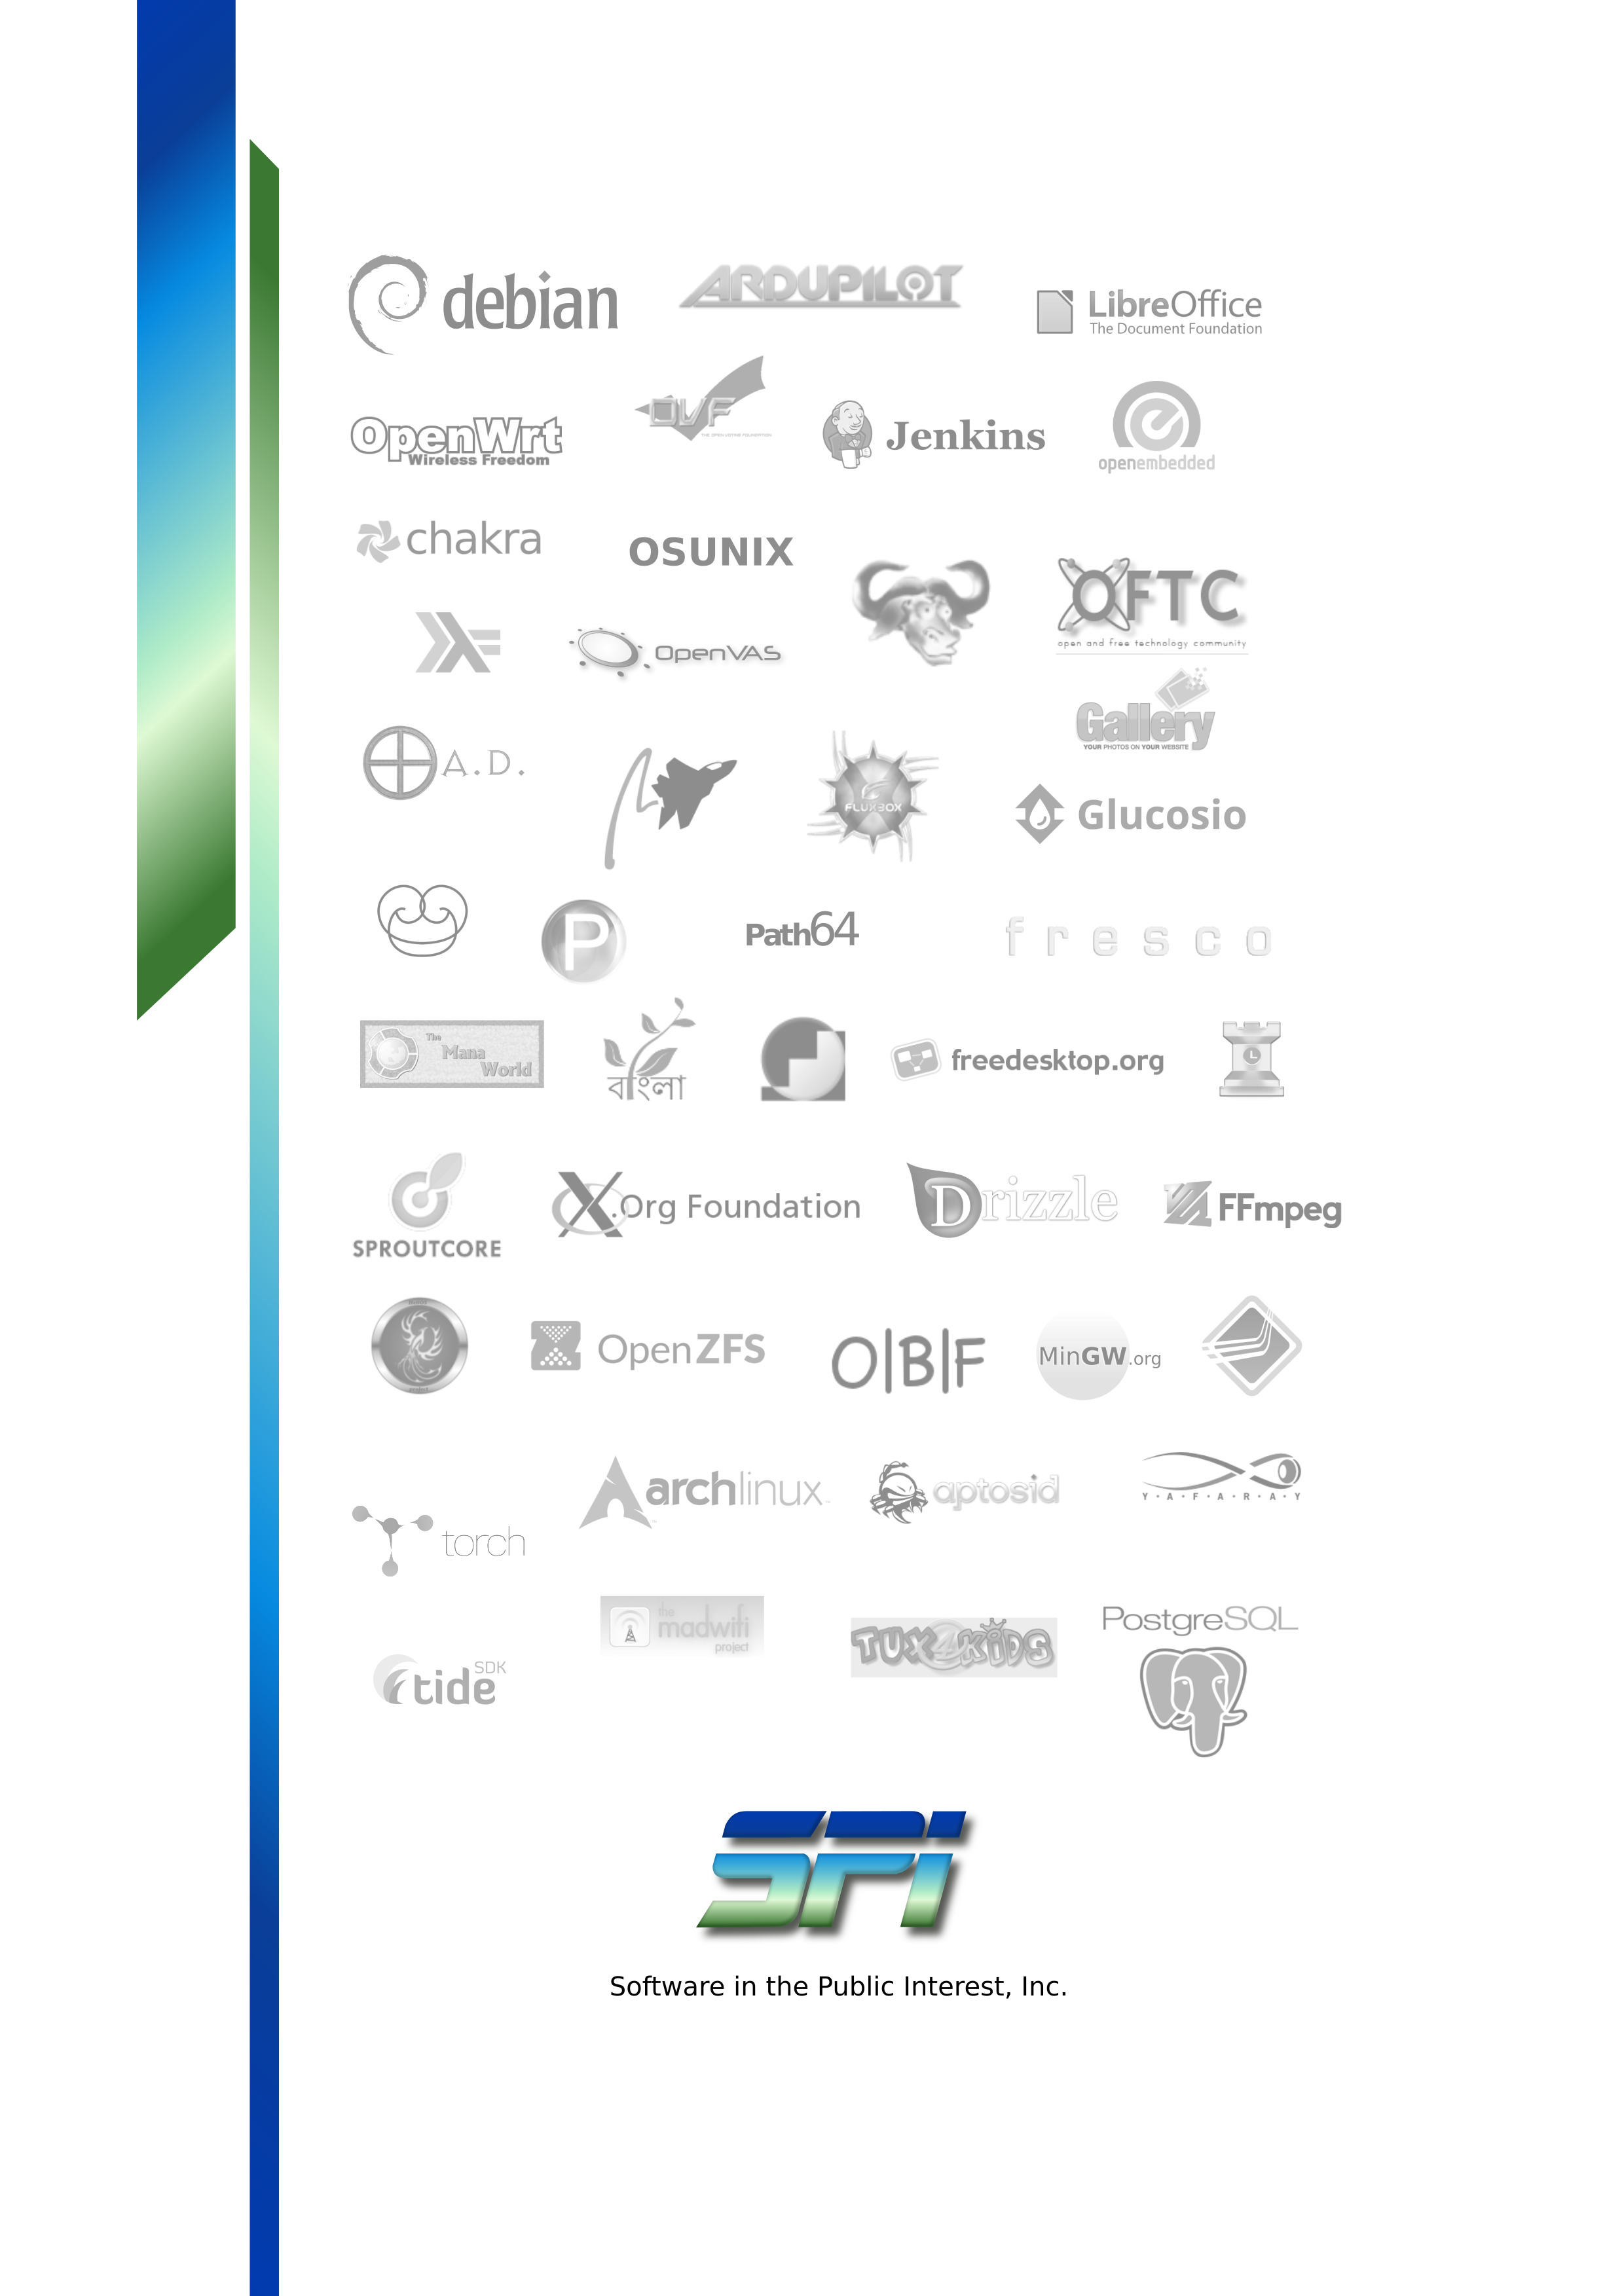
\includegraphics[width=\paperwidth,height=\paperheight]{images/spi-back-2017.jpg}}
}

\null

\end{document}
% Keep this at the bottom, thanks.
% Local Variables:
% TeX-master: "report"
% End:
